%%%%%%%%%%%%%%%%%%%%%%%%%%%%%%%%%%%%%%%%%%%%%%%%%%%%%%%%%%%%%%%%%%%%%%%%%%%%%%%%
% experiment.tex: The CMS detector
%%%%%%%%%%%%%%%%%%%%%%%%%%%%%%%%%%%%%%%%%%%%%%%%%%%%%%%%%%%%%%%%%%%%%%%%%%%%%%%%
\chapter{The CMS Detector}
\label{detector}
%%%%%%%%%%%%%%%%%%%%%%%%%%%%%%%%%%%%%%%%%%%%%%%%%%%%%%%%%%%%%%%%%%%%%%%%%%%%%%%%

The compact muon solenoid (CMS) detector is one of two general-purpose detectors located at the large hadron collider (LHC) near Geneva, Switzerland. The LHC consists of two counter-rotating proton beams in a 27 km ring which cross at several designated points, producing particle collisions with center-of-mass energies near \SI{13.7}{\tera\eV}. 
One of these crossing points is in the center of the CMS detector, where 'bunches' of $\thicksim10^{11}$ protons collide every \SI{25}{\nano\second} in a FIND NUMBER beam spot. 
On average, each bunch crossing has 32 proton-proton interactions, though most are 'pileup' interactions from proton scattering or other unwanted processes.
Occasionally, these collisions will produce exotic, high energy interactions between the quarks within the protons. 
The proton interactions produce large numbers of secondary particles which radiate outward from the beam spot, and the detector measures and identifies these particles in order to reconstruct the physics processes that occurred during the collisions. 
While the bunches interact at a rate of \SI{40}{\mega\hertz}, the large amount of data produced in each collision and the limited data transfer and storage ability limits the final readout to $\thicksim$\SI{1000}{\hertz}.
To obtain this dramatic reduction in event rate, a triggering system is used to rapidly determine 'interesting' events and keep full information from those collisions while discarding any other interactions. 

To successfully achieve these goals, the CMS detector must be able to rapidly identify outgoing particles from a large number of collisions, separate them into individual interactions, determine when physics processes of interest have occurred, and accurately measure and read out all final state particles in triggered events in order to allow for detailed reconstruction. 

The CMS detector consists of several subsystems located concentrically around the collision point. 
Starting from the center, particles first pass through the pixel and strip trackers, which precisely measure the position of charged particles to determine trajectories and vertex locations, as well as their momenta.
Next, particles energy the electromagnetic calorimeter (ECAL) which measures the energy of electrons, photons, and some mesons by completely stopping them through electromagnetic showers and measuring the resulting energy deposits.
After the ECAL, particles enter the hadronic calorimeter (HCAL), which measures neutral hadrons and other less interacting particles which may pass through the ECAL by having many layers of dense absorber to induce hardonic showers interleaved with scintillator layers to measure the resulting energy.
Finally, any remaining particles will pass into the muon chambers, which consist of cathode strips, resistive plates, and gas chambers which all track the motion of muons, as they are the only particles visible to our detector which are unlikely to be stopped in the calorimeters.

In addition to the detecting subsystems, the central feature of the CMS detector is a superconducting solenoid located between the HCAL and muon chambers, which produces a \SI{3.8}{\tesla} magnetic field along the axis of the beam. 
A steel return yoke is located within the muon chambers to capture the fringe field from the solenoid, producing a field in the opposite direction to aid with the measurement of muon momenta.
The large magnetic field provided by the solenoid reduces the neccesary detector size to measure particle momentum and increased resolution of the measured \pt, and the relatively small size of the resulting detector and use of the return yoke for muon measurements give the detector its name.

To best describe particle momenta and take advantage of the nearly cylindrical symmetry of the detector, a special coordinate system is defined. 
The Z-axis is chosen to be oriented along the beam line, and the transverse distance from it is referred to as $\rho$. 
Instead of the polar angle $\theta$, we instead use the pseudorapidity $\eta$. 

\begin{equation}
    \label{eq:pseudo}
    \eta = - log \left[tan\left(\frac{\theta}{2}\right)\right]
\end{equation}

In special relativity, rapidity ($y$) is a measure of relativistic velocity with the feature that differences in rapidity are invariant under Lorentz transformations along the z-axis.
The definition of particle rapidity is shown in \cref{eq:rapidity}, where E is the particle's total energy and p$_z$ is its z-momentum.
\begin{equation}
    \label{eq:rapidity}
    y = \frac{1}{2} ~ln \left(\frac{E+p_z}{E-p_z}\right)
\end{equation}

Pseudorapidity is constructed to form an analogue of rapidity using only geometric information, and converges to match rapidity in the high-energy limit when particle mass is negligible.
Pseudorapidity is zero when perpendicular to the beam, and approaches positive and negative infinity along the z axis. 
By using $\eta$, selections using the angular separation of particles do not have strong dependence on longitudinal momentum and the overall distribution of outgoing collision products is nearly uniform instead of strongly peaked towards zero and $\pi$ as it is using $\theta$.  
The angular distance in this coordinate system is defined as $\Delta R = \sqrt{(\eta_1-\eta_2)^2+(\phi_1-\phi_2)^2}$.

\section{Tracker}
The innermost part of the detector is the CMS tracker, which uses silicon detectors arranged in pixels and strips to measure ionizing radiation from collision products. 
A full description of this detector can be found in Reference \cite{trackerTDR}.
When ionizing particles pass through the silicon sensors, they excite electron-hole pairs within the silicon, which are collected via an applied electic field in the material and produce an output current pulse in the readout electronics.
The positions of these deposits in the silicon are then used to reconstruct the tracks of charged particles.
Using tracks, the charge and momentum of particles can be determined through their curvature in the magnetic field and particle trajectories can be extrapolated to the collision point in order to group tracks from the same interaction into vertices. 
High positional resolution is very important for track reconstruction to resolve individual vertices and separate pileup interactions as well as to precisely determine the track curvature over the length of the tracker. 

The pixel detectors are positioned in the inner part of the CMS tracker, where the high particle density requires the best position resolution. 
The pixel detector was upgraded in 2017 \cite{pixelUpgrade}, and the upgraded version is used for the description here and all of the data samples used. 
The individual pixels are made of 100 $\times$ \SI{150}{\micro\meter} sensors which are placed in three disks in the endcap ($1.5<\lvert\eta\rvert<2.5$) region and four layers in the barrel ($\lvert\eta\rvert<1.5$) region, and have the short axis aligned in the $\phi$ direction so that measurements of curvature in $\phi$ from the magnetic field will have increased resolution from the smaller cell size. 
The resulution is further increased to sub-cell precision through charge-sharing from capacitive coupling to adjacent cells, resulting in final position resolution on the order of \SI{10}{\micro\meter} along the short axis and \SI{20}{\micro\meter} in the longitudinal direction.

In deeper parts of the tracking system, the increased spatial dimension and reduced particle density reduces the need for pixel resolution and instead silicon strips of up to \SI{10}{\centi\meter} in length are used. 
In the barrel region, 10 strip layers are present, reaching up to \SI{110}{\centi\meter} from the beam, and the strips are oriented slightly off-axis in alternating layers to increase the resolution in the z-direction. 
In the endcap, the strips are oriented perpendicularly to the beam in 12 disks up to a radial distance of \SI{270}{\centi\meter}.
Hits in the strip tracker have typical resolutions near \SI{200}{\micro\meter} in the Z-direction and \SI{20}{\micro\meter} in the $\phi$ direction.

The combination of pixel and strip trackers results in very good track reconstruction efficiency and position and momentum resolution.
Muon tracks are reconstructed with $>99\%$ efficiency over the entire $\eta$ range of the tracker, and vertices are reconstructed with resolutions near \SI{50}{\micro\meter}.
Because higher energy tracks have less curvature, the \pt resolution of tracks decreases as the \pt itself increases. Tracks with typical \pt and $\eta$ used in this analysis (\pt near \SI{100}{\giga\eV} and $1.4<\eta<2.4$) have resolutions near 4$\%$. 

\section{ECAL}
The electromagnetic calorimeter sits outside of the tracker, and is split into a barrel and two endcap sections. 
The ECAL barrel covers $\lvert\eta\rvert<$1.479 and $\rho<$\SI{160}{\centi\meter}, while the endcaps cover 1.479$<\lvert\eta\rvert<$3 and $\lvert z \rvert <4$. 
Both sections consist of lead tungstate (PbWO$_4$) crystals, a dense (\SI{8.28}{\gram\per\cubic\centi\meter}) transparent crystal which produces scintillation light when it interacts with a high-energy particle. 
The scintillating radiation is absorbed by Avalanche Photodiodes in the barrel and Vacuum Phototriodes in the endcaps to measure the energy deposited within each 
crystal. 

The crystals are tapered and arranged projectively at a slight angle to minimize inter-crystal gaps, pointing roughly \SI{3}{\degree} away from the collision point. 
They are about 23 cm, or 25 $X_0$, in depth, and have a transverse size of 2.2 $\times$ \SI{2.2}{\centi\meter^2} in the barrel and 2.9$\times$\SI{2.9}{\centi\meter^2} in the endcap. 
Each endcap is divided vertically into two 'Dees', each with 3660 crystals grouped into 5x5 units called 'Supercrystals'. 
During 2018 data taking, several supercrystals within the ECAL endcaps observed problems during data quality monitoring, and were 'masked' to remove their measurements from the total energy sums \cref{fig:EEmasks}, removing roughly 2$\%$ of the total ECAL area.
To avoid potential backgrounds from tracks with missing energy from showers in these masked regions, signal tracks are required to have $\Delta R>0.1$ to any masked supercrystal.

\begin{figure}[h]
    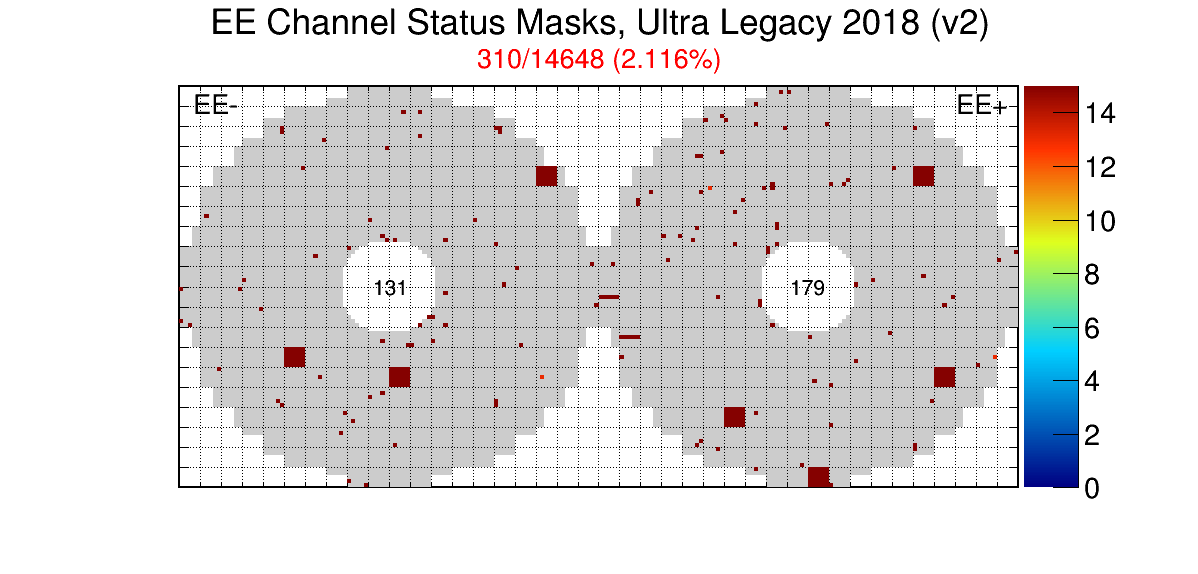
\includegraphics[width=0.9\textwidth]{figures/EEChannelMasks.png}
    \centering
    \caption{EE Channel Masks in Ultra Legacy 2018 MC Conditions \cite{EcalDPG}.}
    \label{fig:EEmasks}
\end{figure}

\section{HCAL}
The CMS hadronic calorimeter (HCAL) is a sampling calorimeter, which consists of alternating layers of brass absorber and plastic scintillator. 
Hadronic showers are primarily induced in the absorber, and the energy of the shower is sampled in each layer of scintillator and the sampled energy is used to estimate the total energy of the shower. 
While this method of sampling significantly lowers the precision of the energy measurement, it allows most of the detector material to be made of relatively cheap absorber instead of scintillating material, which results in a very substantial cost difference due to the large amount of material required to stop high-energy hadrons.
The HCAL endcaps have 17 active layers of plastic scintillator and \SI{8}{\centi\meter} absorber, covering 1.4$<\eta<$2.4 and extending to $\lvert z \rvert<$ \SI{5.6}{\meter}, with a total radiation length near 200 X$_0$. 
The thickness of ECAL and HCAL is sufficient to stop nearly all mesons and hadrons produced in the collision, leaving only neutrinos, which are not visible in the detector, and muons. 
The scintillaton light from the sampling layers is collected in wavelength-shifting fibers, then transported to readout electronics.
This light collection is done in the HCAL barrel (and Endcaps, prior to 2018) by hybrid photodiodes (HPDs). 
During readout, scintillation light from successive HPDs is summed together into 'towers', reducing the available depth information to one or two depths, depending on the detector location.

In the ECAL endcap, radiation damage to the scintillating tiles caused by high particle flux neccesitated the replacement of the avalanche photodiodes with silicon photomultipliers (SiPMs) in 2018, which have three times better photon detection efficiency than HPDs.  
The SiPMs also have smaller footprints than the HPDs, allowing for more of them to be placed in the volume previously occupied by the HPDs and reducing the need for depth summation before readout. 
Using this, energy information from HE after the SiPM installation is now grouped into 6-7 depths as shown in \cref{fig:HElayout}.

\begin{figure}[!htpb]
	   \centering
	      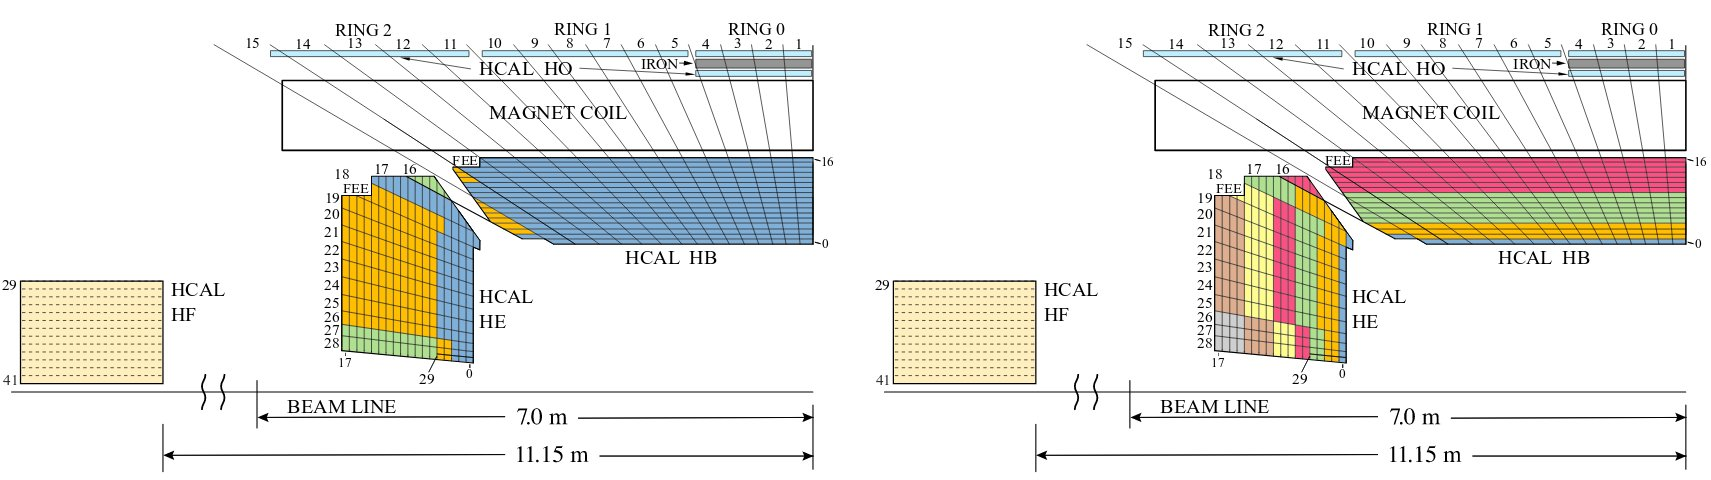
\includegraphics[width=\textwidth]{figures/HE_upgrade.jpg}
		 \caption[The 2018 HE upgrade]{The CMS HCAL geometry before (left) and after (right) the SiPM installation. Each rectangle represents a cell, and like-colored cells in HCAL at each i$\eta$ and i$\phi$ are summed to create a 'hit' at the depth represented by their color. These hits are the most granular HE information available. As the upgrade was only performed in HE for 2018 data taking, individual depth information is only available in the endcap for this analysis.}
	    \label{fig:HElayout}
\end{figure}

As a consequence of the improved photon resolution from the HPD replacement, muon energy deposits are now visible in HE when they were below the noise floor for the HPDs. 
This, in addition to the improved depth segmentation, provide very powerful tools for separating muon tracks from backgrounds as well as observing potential disappearance events.
Potential signal tracks are thus required to be in the endcap, as the barrel regions do not have the resolution to effectively observe muons or reject missing energy from standard model processes or non-muon tracks.

In the readout chain, the HCAL sensors are grouped into 'sectors' containing clusters of cells. During the 2018 data taking two sectors could not be operated, resulting an a roughly 40 degree section with effectively no HCAL information. Similiarly to the inactive ECAL regions, these inoperable sectors could result in missing energy from showers within them, and so nearby tracks are excluded from the search. 
To avoid these regions, all signal tracks are required to be outside of the region of -3.0$<\eta<$ -1.3 and -1.57$<\phi<$-0.87, removing roughly 10$\%$ of potential tracks.

\section{Muon Systems}
